\documentclass[a0,portrait]{a0poster}

%--------------------
\newlength{\sepwidth}
\setlength{\sepwidth}{3.5cm}

\newlength{\colwidth}
\setlength{\colwidth}{22.32cm}

\newlength{\twocolwidth}
\setlength{\twocolwidth}{48.14cm}
%--------------------

\usepackage{wrapfig}
\usepackage[svgnames]{xcolor}
\usepackage{graphicx} 
\usepackage{amsfonts, amsmath, amsthm, amssymb}

\usepackage[font=small,labelfont=bf]{caption}

\usepackage{algorithm} 
\usepackage{algpseudocode}
\usepackage{wrapfig}

\newcommand{\fspic}[3][1] {
  \begin{center}\vspace{1cm}
    \includegraphics[width=#1\linewidth]{pics/#2}
    \captionof{figure}{#3}
    \label{#1}
  \end{center}\vspace{1cm}
}

\newcommand{\fssection}[3] {
  \section*{#1}
}

\newcommand {\FlameStream} {FlameStream}

\begin{document}

  \begin{minipage}[t]{.86\linewidth}
    {\huge \textbf{\FlameStream: Model and Runtime for Distributed Stream Processing}}\\
    \bigbreak
    {\large \textbf{Igor E. Kuralenok$^1$, Artem Trofimov$^{1,2}$, Nikita Marshalkin$^{1,2}$, and Boris Novikov$^{1,2}$}}\\
    \bigbreak
    {\large $^1$JetBrains Research, $^2$Saint Petersburg State University}
  \end{minipage}
  %
  \begin{minipage}[t]{0.14\linewidth}
    
\includegraphics[width=10cm]{pics/jetbrains.png} 
  \end{minipage}

  \vspace{3cm}

  \begin{minipage}[t]{\twocolwidth}
    \centering
    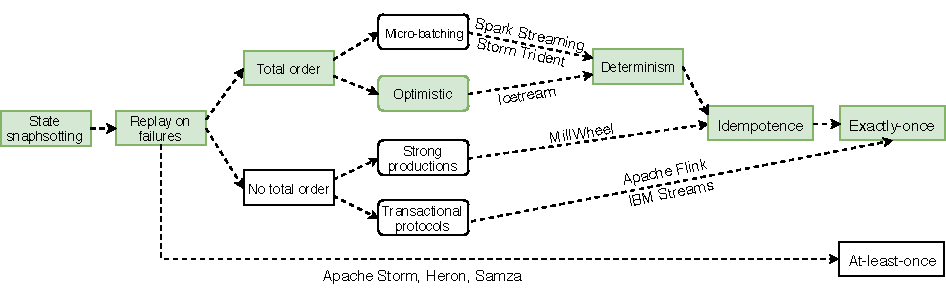
\includegraphics[width=\linewidth]{pics/roadmap}
    \captionof{figure}{The roadmap of approaches for achieving exactly-once and at-least-once guarantees. Green elements indicate the path for our approach}
  \end{minipage}
  %
  \hspace{\sepwidth}
  %
  \begin{minipage}{\colwidth}
    \fssection{Garbage filtering}
    In case of reordering invalid tuples are generated. In order to return only correct tuples to users there is a barrier at the end of the pipeline. It passes correct items and filters out incorrect ones.

    \fspic{happy-man}{Barrier collects elements in a buffer and removes items if corresponding tombstones have arrived. It flushes buffer periodically and returns elements to the end-user. Punctuations (low-watermarks) proposed in OOP approach can be used as a flush-trigger}
  \end{minipage}

  \vspace{1cm}

  \begin{minipage}[t]{\colwidth}
    \fssection{Graph as a function}

    Determenistic exactly-once processing makes execution results predictable and repeatable as they are completely determined by input elements and a logical graph. This property is useful for preserving strong consistency in presence of failures and recoveries, because input replay does produce exactly the same results regardless the asynchronous nature of distributed systems. 

    \fspic{function}{If computations are determenistic idempotance can be achieved by deduplication buffer at the end of a pipeline}

    \fssection{Drifting state}
    Effectively, modern stream processing models allows managing an operation state in a form of  
    
    \[(in, state) \rightarrow (out, newState)\]
    
    Even if systems do not provide such interface explicitly, it is implemented internally and exported via consistent state wrappers. We make such contract explicit by decomposing any stateful operation into two operations with a cycle:

    \fspic{transition}{Any stateful transformation can be expressed by a combination of windowed grouping and stateless map operations}

    \begin {description}
      \item [Map] applies a user-defined function to the payload of an input item and returns a (possibly empty) sequence of data items with transformed payloads. 
      \item [Grouping] constructs a single item containing a set of consecutive items that have the same value of partition function. The maximum number of items that can be grouped is specified as a parameter  $Window Size.$ 
    \end{description}

    Groupings of different partitions are independent.
  \end{minipage}
  %
  \hspace{\sepwidth}
  %
  \begin{minipage}[t]{\twocolwidth}
    \begin{minipage}[t]{\colwidth}
      \fssection{Ordering}
      To achieve deterministic results and to properly manage drifting state cycles, there is a need to impose strong processing order on data items.

      \fspic{ordering}{Data item with payload $1'$ is the derivative of the item with payload $1$, according to operation $F$. The same is for items with payloads $2'$ and $2$. After merge operation, the order between $1$ and $2$ is preserved. Furthermore, $1'$ follows $1$, and $2'$ follows $2$.}

      \fssection{Optimistic out-of-order processing}
      To achieve system-wide ordering, it is sufficient to impose strong order only within grouping operations. 
      
      Grouping state has a well-defined simple structure that allows handling out-of-order items speculatively without extra buffering. More precisely, grouping immediately processes input items as they were in-order. In case of reordering, it is locally generates correct tuples and sends tombstones for incorrect ones. 
      \fspic{grouping-invalidation}{On arrival of out-of-order item, it is inserted in the correct location of the correcponding bucket. Valid elements containing new item are produced, and invalid ones are invalidated by sending a tombstone for it down the stream}

    Within the  optimistic approach, we accept the fact that grouping can produce incorrect output, but we guarantee that all correct groups are eventually produced.  
    \end{minipage}
    %
    \hspace{\sepwidth}
    %
    \begin{minipage}[t]{\colwidth}
      \fssection{Consistency}
      The properties of the proposed model lay the foundations for providing exaclty-once semantics with low overhead. Total order and determinism allows filtering out duplicates at the barrier by comparing timestamps. Grouping state structure enables performing asynchronous snapshots. 

     Therefore, our architecture decouples result releasing and state snapshotting mechanisms. Hence, it does not require heavy transactional protocols for achieving exactly-once.

      \fspic[.7]{bucket-parts}{Grouping buckets can be divided into the two parts: immutable and mutable. The separator is the time of the last received punctuation (we call it minimal time). State snapshot for any time before the minimal can be obtained by cutting window-sized sublist}

      \vspace{1cm}

      \fssection{Experiments}
      We used a problem of building an incremental inverted index as a stream processing benchmark.

      The latency is defined as a (negated) time difference between the entry of new page and the delivery of all index updates generated in response.

      Our experiments were performed on the cluster of Amazon EC2 micro instances with 1GB RAM and 1 core CPU. We used 10000 Wikipedia articles as a dataset. 
    \end{minipage}

    \vspace{1cm}

    \begin{minipage}[t]{\linewidth}
      \fspic{comparison}{Comparison}
    \end{minipage}
  \end{minipage}

  \begin{minipage}{\linewidth}
    \begin{center}
      
\includegraphics[width=.05\linewidth]{pics/qr-code}
    \end{center}
  \end{minipage}
\end{document}
